\documentclass[usenames,dvipsnames,letterpaper, reqno,11pt]{article}
\usepackage[margin=1.0in]{geometry}
\usepackage{color,latexsym,amsmath,amssymb, amsthm, graphicx,subfigure}

\usepackage{amsthm}
\usepackage{amsmath}
\usepackage{multicol}
\usepackage{amssymb}
\usepackage{mathabx}
\usepackage{accents}
\usepackage[english]{babel}
\usepackage{blindtext}
\usepackage{graphicx}
\usepackage{multicol}

\usepackage{tikz}
\usepackage{tkz-berge}
\usepackage{tkz-graph}

\usetikzlibrary{patterns,arrows,decorations.pathreplacing}

\usepackage{xcolor}
\definecolor{dblue}{RGB}{20,66,129}
\definecolor{rose}{RGB}{255,101,122}
\definecolor{crimsonred}{RGB}{132,22,23}
\definecolor{darkblue}{RGB}{72,61,139}

\definecolor{deepblue}{RGB}{36,123,160}
\definecolor{deepred}{RGB}{255,22,84}
\definecolor{deeporange}{RGB}{240,111,62}

\definecolor{olive}{rgb}{0.3, 0.4, .1}
\definecolor{fore}{RGB}{249,242,215}
\definecolor{back}{RGB}{51,51,51}
\definecolor{title}{RGB}{255,0,90}
\definecolor{dgreen}{rgb}{0.,0.6,0.}
\definecolor{gold}{rgb}{1.,0.84,0.}
\definecolor{JungleGreen}{cmyk}{0.99,0,0.52,0}
\definecolor{BlueGreen}{cmyk}{0.85,0,0.33,0}
\definecolor{RawSienna}{cmyk}{0,0.72,1,0.45}
\definecolor{Magenta}{cmyk}{0,1,0,0}





\theoremstyle{plain}
\newtheorem{lemma}{Lemma}
\newtheorem{prop}{Proposition}
\newtheorem*{example}{Example}
\newtheorem*{fact}{Fact}
\newtheorem{corollary}{Corollary}

\usepackage{algorithm}
\usepackage[noend]{algpseudocode}

\theoremstyle{plain}
\newtheorem{theorem}{Theorem}
\newtheorem{proposition}[theorem]{Proposition}
\newtheorem*{remark}{Remark}

\def\changemargin#1#2{\list{}{\rightmargin#2\leftmargin#1}\item[]}
\let\endchangemargin=\endlist 

\DeclareMathOperator{\codim}{codim}
\DeclareMathOperator{\lhdim}{\underline{\dim}_{\mathbf{M}}}
\DeclareMathOperator{\lmbdim}{\underline{\dim}_{\mathbf{MB}}}
\DeclareMathOperator{\biggercup}{\mathbin{\bigcup}}%


\newcommand{\RR}{\mathbb{R}}

\title{Large Sets Avoiding Rough Patterns}
\author{Jacob Denson\thanks{University of British Columbia, Vancouver BC, \{denson, malabika, jzahl\}@math.ubc.ca.} \and Malabika Pramanik\footnotemark[1] \and Joshua Zahl\footnotemark[1]}

\begin{document}

\maketitle










\begin{abstract}
	The pattern avoidance problem seeks to construct a set $X\subset \RR^d$ with large dimension that avoids a prescribed pattern such as $x_1-2x_2+x_3=0$ (i.e. three term progressions), or more general patterns such as $f(x_1,\ldots,x_n)=0$. Previous work on the subject has considered patterns described by polynomials, or by functions $f$ satisfying certain regularity conditions. We consider the case of ``rough'' patterns. There are several problems that fit into the framework of rough pattern avoidance. As a first application, if $Y\subset[0,1]$ is a set with Minkowski dimension $\alpha$, we construct a set $X\subset[0,1]$ with Hausdorff dimension $1-\alpha$ so that $X+X$ is disjoint from $Y$. As a second application, given a set $Y$ of dimension close to one, we can construct a subset $X\subset Y$ of dimension $1/2$ that avoids isosceles triangles. [{\bf{TODO:}} I'd like to replace this with a rectifiability statement]
\end{abstract}



A key question in modern geometric measure theory and additive combinatorics is how dense a set can be before certain patterns are forced to occur. One of the foundational results in this area is Roth's theorem in additive combinatorics. In \cite{Roth}, Roth proved an ``existence'' result for three-term arithmetic progressions; he showed that if $X\subset[N]$ satisfies $|X|\geq CN/\log\log N$ for some sufficiently large absolute constant $C$, then $X$ must contain a three-term arithmetic progression. In the opposite direction, Behrend \cite{Behrend} established an ``avoidance'' result for three-term arithmetic progressions; he constructed a set $X\subset[N]$ with $|X|\geq N\exp(-c\sqrt{\log N})$ that does not contain any three-term arithmetic progressions. While Roth's bound has seen subsequent improvements, the precise density threshold at which three-term arithmetic progressions are forced to occur remains unknown. 

There are a number of problems in geometric measure theory that may be viewed as continuum analogues of the avoidance problem described above. Here one considers (infinite) sets $X\subset\RR$ rather than finite sets of integers, and the notion of density is replaced by that of dimension. For example Keleti \cite{KeletiDimOneSet} constructed a compact subset of $\RR$ with Hausdorff dimension one that contains no ``one-dimensional parallelogram" and in particular, no three-term arithmetic progressions. Four points $x_1<x_2 \leq x_3 < x_4$ form a one-dimensional parallelogram precisely when $x_2-x_1 = x_4-x_3$. In \cite{Mathe}, M\'ath\'e considered the avoidance problem for a countable family of polynomial patterns of the form $f(x_1, \cdots, x_n) = 0$, while in \cite{MalabikaRob}, Fraser and the second author considered a related avoidance problem where the functions $f$ are smooth and only need to satisfy mild nondegeneracy conditions.

Observe that if $Z = \{(x_1,x_2,x_3, x_4)\in\RR^4 \colon x_2- x_1 - x_4 + x_3 =0\}$, then a set $X\subset\RR$ avoids a nontrivial one-dimensional paralleogram precisely when the intersection $X^4\cap Z$ consists only of points $(x_1,x_2,x_3, x_4)$ where two or more coordinates are equal. Generalizing this, suppose that $f: \mathbb R^{nd} \rightarrow \mathbb R$ is a function that vanishes on the union of the planes $\{(x_1, \cdots, x_n) \in (\mathbb R^d)^n : x_i = x_j \text{ for some choice of } i \neq j \}$. If $Z = \{x_1,\ldots,x_n)\in\RR^{dn}\colon f(x_1,\ldots,x_n)=0\}$, then we say that $X\subset\RR^d$ avoids the pattern $f(x_1,\ldots,x_n)=0$ precisely when the intersection $X^n\cap Z$ consists only of points $(x_1,\ldots,x_n)$ where two or more coordinates are equal. In this framework, M\'ath\'e \cite{Mathe} constructed a set $X$ that avoids a countable union of algebraic varieties, while Fraser and the second author \cite{MalabikaRob} constructed a set $X$ avoiding a countable union of smooth varieties of finite type.

In this paper, we consider a version of the avoidance problem for ``rough'' sets $Z\subset\RR^{dn}$ that are obtained by taking a countable union of sets, each with controlled lower Minkowski dimension. In contrast with previous work, no further assumptions are made on $Z$. The dimension of our avoiding set $X\subset\RR^d$ will depend only on the ambient dimension $d$, the number of variables $n$, and the lower Minkowski dimension of the sets in $Z$. A precise version of our result is given below. 



\begin{theorem}\label{mainTheorem}
	Let $d\leq\alpha<dn$ and let $Z \subset \RR^{dn}$ be a countable union of compact sets, each with lower Minkowski dimension at most $\alpha$. Then there exists a set $X \subset [0,1]^d$ of Hausdorff dimension $\frac{nd - \alpha}{n-1}$ such that whenever $x_1, \dots, x_n \in X$ are distinct, we have $(x_1, \dots, x_n) \not \in Z$.
\end{theorem}

Note that when $\alpha<d$ the pattern avoidance problem is trivial, since we can simply select $X = [0,1]^d\ \backslash\ \pi(Z)$, where $\pi\colon\RR^{dn}\to\RR^d$ is the projection to the first coordinate. This choice of $X$ will have Hausdorff dimension $d$ and will satisfy the conclusions of Theorem \ref{mainTheorem}. The case $\alpha=dn$ is trivial as well, since $X=\emptyset$ satisfies the conclusions of Theorem \ref{mainTheorem}.

When $Z$ is a countable union of smooth manifolds, Theorem \ref{mainTheorem} generalizes Theorems 1.1 and 1.2 from \cite{MalabikaRob}. In Section \ref{futureWorkSection} we compare our methods with those in \cite{MalabikaRob}, as well as other pattern avoidance methods. Theorem \ref{mainTheorem} also allows us to find large subsets of arbitrary sets that avoid prescribed patterns. Specifically, if $Y\subset\RR^d$ and $Z\subset\RR^{dn}$, we can find a subset $X\subset Y$ of large dimension so that $X^n$ avoids $Z$. This will be discussed further in Section \ref{applicationsSection}.


Theorem \ref{mainTheorem} is proved using a Cantor-type construction, a common theme in the surrounding literature. For a sequence of decreasing length scales $\ell_n \rightarrow 0$ to be chosen, the construction specifies a selection mechanism for generating a nested sequence of sets $X_n$.  The set $X_n$ obtained at the $n$-th step is a union of cubes of sidelength $\ell_n$, and avoids $Z$ at scales close to $\ell_n$. For each $n$, the selection proceeds through a three-scale randomized construction adapted to the scale $\ell_n$ and involves two auxiliary scales $r_n$ and $s_n$ (the scale $s_n$ will later become the scale $\ell_{n+1}$). This randomized construction, described in Section \ref{sinceScaleSection}, is an important contribution of this paper. On one hand, the selection mechanism assigns mass uniformly on intermediate auxiliary scales, akin to \cite{MalabikaRob}, eventually ensuring large Hausdorff dimension. On the other hand, the randomization allows us to avoid the complicated queueing techniques in \cite{{KeletiDimOneSet}, {MalabikaRob}}. In Section \ref{multiScaleSection}, we employ a multi-scale analysis to combine the sets $X_n$ into a single set $X$ that avoids $Z$ at all scales. Finally, in Section \ref{dimensionBoundSection} we analyze our construction and show that the resulting set $X$ has the correct Hausdorff dimension. 




\section{Frequently Used Notation and Terminology}

\begin{itemize}
	\item For a length $\ell>0$, let $\mathcal{B}^d_\ell$ denote the set of all half open cubes in $\RR^d$ with side length $\ell$ and corners on the lattice $(\ell \cdot \mathbf{Z})^d$. That is,
	%
	\[ \mathcal{B}^d_\ell = \{ [a_1,a_1 + \ell) \times \dots \times [a_d, a_d + \ell) : a_i \in \ell \cdot \mathbf{Z} \}. \]
	%
	If $E \subset \RR^d$, define $\mathcal{B}^d_\ell(E)$ to be the family of cubes in $\mathcal{B}^d_\ell$ intersecting $E$, i.e.
	%
	\[\mathcal{B}^d_\ell(E) = \{ I \in \mathcal{B}^d_\ell: I \cap E \neq \emptyset \}. \]

	\item The {\it lower Minkowski dimension} of a compact set $E \subset \RR^d$ is
	%
	\[ \lhdim(E) = \liminf_{\ell \to 0} \frac{\log( \#( \mathcal{B}^d_\ell(E) ) )}{\log(1/\ell)}. \]

	\item A {\it dyadic scale} is a length $\ell = 2^{-k}$ for some non-negative integer $k$.

	\item A {\it Frostman measure} of dimension $\alpha$ is a compactly supported positive finite Borel measure $\mu$ on $\RR^d$ for which there exists a constant $C > 0$ with the following property: $\mu(B(x;r)) \leq C r^\alpha$ for any ball $B(x;r) \subseteq \mathbb R^d$. This is equivalent to the requirement that for some constant $C > 0$ any dyadic scale $\ell$, and any cube $I \in \mathcal{B}^d_\ell$, we have $\mu(I) \leq C \ell^\alpha$.

	\item The {\it Hausdorff dimension} of a set $X \subset \RR^d$ is
	%
	\[ \dim_{\mathbf{H}}(X) = \sup \left\{ \alpha: \begin{array}{c} \text{There is an}\ \alpha\ \text{dimensional Frostman}\\
	\text{measure supported on $X$} \end{array} \right\}. \]

	\item Adopting the terminology of \cite{KatzTao}, we say a collection of distinct sets $U_1, U_2, \dots$ is a {\it strong cover} of a set $E$ if $E \subset \limsup U_k$, which means every element of $E$ is contained in infinitely many of the sets $U_k$.

	\item Given $I \in \mathcal{B}^{dn}_\ell$, we can decompose $I$ as $I_1 \times \dots \times I_n$ for unique cubes $I_1, \dots, I_n \in \mathcal{B}^d_\ell$. We say $I$ is {\it strongly non-diagonal} if the cubes $I_1, \dots, I_n$ are distinct.
\end{itemize}










\section{Avoidance at Discrete Scales}\label{sinceScaleSection}
In this section we will describe a method for avoiding $Z$ at a single scale. In the next section, we will analyze $Z$ at many scales to construct a set $X$ that avoids $Z$ at all scales. Fix two dyadic scales $\ell$ and $s$, with $\ell > s$. In the discrete setting, we replace $Z \subseteq \mathbb R^{dn}$ by a union of cubes in $\mathcal B_s^{dn}$, denotes $Z_s$, that covers $Z$. Given a set $E$, which is a union of cubes in $\mathcal B_{\ell}^d$, our goal is to construct a set $F \subset E$ that is a union of cubes in $\mathcal B_s^{d}$, so that $F^n$ is disjoint from the strongly non-diagonal cubes of $Z_s$.

In order to ensure that our final set $X$ has large Hausdorff dimension, it is crucial that $F$ is spread uniformly over $E$. We achieve this decomposing $E$ into sub-cubes in $\mathcal B_r^{d}$ for some intermediate scale $r \in (s, \ell)$, and distributing $F$ evenly among almost all of these intermediate sub-cubes. The following lemma makes this precise. 

\begin{figure}[h!]
	\centering
    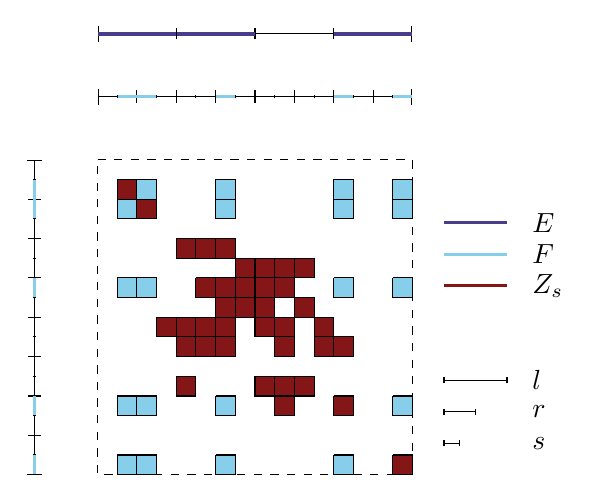
\begin{tikzpicture}[scale=4] %% Change scaling as needed
        \draw [|-]  (0,0) -- (1/4,0);
		\draw (0,0) -- (1,0);
        \draw [-|] (3/4,0) -- (1,0);% node [anchor = south west] {$E$};

        \foreach \x in {1,2,3}
        	\draw (\x/4,-0.5pt) -- (\x/4,0.5pt);

        \foreach \x in {0,1,3}
    		\draw[darkblue, ultra thick] (\x/4+0.001,0) -- (\x/4 + 1/4-0.001,0);




        \draw [|-]  (0,-0.2) -- (1/4,-0.2);
        \draw (0,-0.2) -- (1,-0.2);
        \draw [-|] (6/7,-0.2) -- (1,-0.2);% node [anchor = north west] {$F$};

        \foreach \x in {1,...,15}
            \draw (\x/16,-0.2-0.005) -- (\x/16,-0.2+0.005);

        \foreach \x in {1,...,7}
            \draw (\x/8,-0.2-0.02) -- (\x/8,-0.2+0.02);

        \foreach \x in {1,2,6,12,15}
            \draw[SkyBlue, very thick] (\x/16+0.001,-0.2) -- (\x/16 + 1/16 - 0.001,-0.2);








        \draw [|-]  (-0.2,-0.4) -- ++(0,-0.01);
        \draw (-0.2,-0.4) -- (-0.2,-1.4);
        \draw [-|] (-0.2,-1.38) -- (-0.2,-1.4);% node [anchor = north east] {$F$};

        \foreach \x in {1,...,15}
            \draw (-0.2-0.005,-0.4-\x/16) -- (-0.2+0.005,-0.4 -\x/16);

        \foreach \x in {1,...,7}
            \draw (-0.2-0.02,-0.4-\x/8) -- (-0.2+0.02,-0.4-\x/8);

        \foreach \x in {1,2,6,12,15}
        	\draw[SkyBlue, very thick] (-0.2,-0.4-\x/16-0.001) -- (-0.2,-0.4-\x/16-1/16+0.001);





        \draw[dashed] (0,-0.4) -- (1,-0.4) -- (1,-1.4) -- (0,-1.4) -- (0,-0.4);

        \foreach \x in {1,2,6,12,15}
        	\foreach \y in {1,2,6,12,15}
        		\draw[fill=SkyBlue] (\x/16,-0.4 - \y/16) -- ++(0,-1/16) -- ++ (1/16,0) -- ++(0,1/16) -- ++(-1/16,0);

        \foreach \x in {1,2,6,12,15}
        	\draw[fill=crimsonred] (\x/16,-0.4 - \x/16) -- ++(0,-1/16) -- ++ (1/16,0) -- ++(0,1/16) -- ++(-1/16,0);

        \foreach \x/\y in {4/4, 5/4, 6/4, 7/5, 8/5, 9/5, 10/5, 5/6, 6/6,7/6,8/6,9/6, 6/7, 7/7, 8/7, 10/7, 3/8, 4/8, 5/8, 6/8, 8/8, 9/8, 11/8, 4/9, 5/9, 6/9, 9/9, 11/9, 12/9, 4/11, 8/11, 9/11, 10/11, 9/12}
        	\draw[fill=crimsonred] (\x/16,-0.4 - \y/16) -- ++(0,-1/16) -- ++ (1/16,0) -- ++(0,1/16) -- ++(-1/16,0);







            \draw [darkblue, very thick] (1.1,-0.6) -- (1.3,-0.6);
%            \foreach \x in {1.1, 1.3}
%                \draw (\x,-0.6 - 0.01) -- (\x,-0.6 + 0.01);
            \draw (1.35,-0.6) node [anchor = west] {$E$};

            \draw [SkyBlue, very thick] (1.1,-0.7) -- (1.3,-0.7);
%            \foreach \x in {1.1,1.3}
%                \draw (\x,-0.7 - 0.01) -- (\x, -0.7 + 0.01);
            \draw (1.35,-0.7) node [anchor = west] {$F$};

            \draw [crimsonred, very thick] (1.1,-0.8) -- (1.3,-0.8);
%            \foreach \x in {1.1,1.3}
%                \draw (\x,-0.8 - 0.01) -- (\x, -0.8 + 0.01);
            \draw (1.35,-0.8) node [anchor = west] {$Z_s$};

            \draw (1.1,-1.1) -- (1.3,-1.1);
            \foreach \x in {1.1, 1.3}
                \draw (\x,-1.1 - 0.01) -- (\x,-1.1 + 0.01);
            \draw (1.35,-1.1) node [anchor = west] {$l$};

            \draw (1.1,-1.2) -- (1.2,-1.2);
            \foreach \x in {1.1, 1.2}
                \draw (\x,-1.2 - 0.01) -- (\x,-1.2 + 0.01);
            \draw (1.35,-1.2) node [anchor = west] {$r$};

            \draw (1.1,-1.3) -- (1.15,-1.3);
            \foreach \x in {1.1, 1.15}
                \draw (\x,-1.3 - 0.01) -- (\x,-1.3 + 0.01);
            \draw (1.35,-1.3) node [anchor = west] {$s$};
	\end{tikzpicture}
	\caption{An example depicting a possible choice of $F$ that satisfies the conclusions of Lemma 1 where $d = 1$ and $n = 2$. $F$ satisfies the non-concentration and avoidance property, as well as containing an interval from all but 3 of the intervals in $\mathcal{B}^d_r(E)$.}
\end{figure}
%TODO: Make figure into two-or three distinct figures indicating the process.

\begin{lemma}\label{discreteScaleLem}
	Fix three dyadic lengths $\ell > r > s$. Let $E$ be a union of cubes in $\mathcal{B}^d_\ell$ and let $Z_s$ be a union of cubes in $\mathcal{B}^{dn}_s$. Then there exists $F \subset E$, which is a union of cubes in $\mathcal{B}^d_s$, such that
	%
	\begin{itemize}
		\item[(A)] \emph{Avoidance}:  For any distinct $I_1, \dots, I_n \in \mathcal{B}^d_s(F)$, we have $I_1 \times \dots \times I_n \not \in \mathcal{B}^{dn}_s(Z_s)$.
		\item[(B)] \emph{Non-concentration}: For each cube $I \in \mathcal{B}^d_r(E)$, there is at most one cube $J\in \mathcal{B}^d_s(F)$ with $J\subset I$. 
		\item[(C)] \emph{Large size}: $\# \mathcal{B}^d_s(F) \geq \# (\mathcal{B}^d_r(E)) - |Z_s| r^{-dn}$.
	\end{itemize}
\end{lemma}
\begin{proof}

First, we can assume that $r^{dn}(\# \mathcal{B}^d_r(E))> |Z_s|$, since if this inequality fails then we can take $F=\emptyset$. 

For every $I \in \mathcal B_r^d(E)$, we select, independently and with uniform probability, a sub-cube $J_I \in \mathcal B_s^{d}(I)$. Let $U$ be a random set thus obtained, i.e., 
	%
	\[ U = \bigcup\; \{ J_I: I \in \mathcal{B}^d_r(E) \}. \]
	%
By construction, there is exactly one cube $J \in \mathcal B_s^d(U)$ for each cube $I \in \mathcal B_r^d(E)$. Thus $U$ obeys the requirement of item (B). It also meets the requirement of item (C) trivially, since \begin{equation} \label{UE} \# (\mathcal{B}^d_s(U)) = \# (\mathcal{B}^d_r(E)) \quad \text{ for every $U$}. \end{equation}  However, $U$ may not satisfy item (A). We will show that with non-zero probability, we can find a suitable $U$, modify it by removing at most $|Z_s|r^{-dn}$ cubes from it, so that the resulting set satisfies all three required criteria.  

	Note that for each cube $J \in \mathcal{B}^d_s(E)$, there is a unique ``parent'' cube $I \in \mathcal{B}^d_r(E)$ such that $J \subset I$. Thus for each fixed cube $J \in \mathcal{B}^d_s(E)$
	%
	\[ \mathbf{P}(J \subset U) = \mathbf{P}(J_I = J) = (s/r)^d. \]
	%
	Since any two cubes in $\mathcal{B}^d_s(U)$ are contained in distinct cubes of $\mathcal{B}^d_r$, the only way that a {\it strongly non-diagonal} cube $K = J_1 \times \dots \times J_n\in\mathcal{B}^{dn}_s(Z_s)$ is a subset of $U^n$ is if each of the cubes $J_1, \dots J_n$ are contained in distinct cubes of $\mathcal{B}^d_r$. Since the events that each cube $J_k$ is contained in $U$ are independent, we have that
	%
	\begin{align*}
		\mathbf{P}(K \subset U^n) &= \mathbf{P}(J_1 \subset U) \cdots \mathbf{P}(J_n \subset U) = (s/r)^{dn}.
	\end{align*}
	%
	Let $\mathcal{K}(U)$ denote the family of all strongly non-diagonal cubes $K \in \mathcal{B}^{dn}_s(Z_s)$ contained in $U^n$. Letting $K$ range over the strongly non-diagonal cubes of $\mathcal{B}^{dn}_s(Z_s)$, we conclude that
	%
	\begin{align*}
		\mathbf{E}(\# (\mathcal{K}(U))) &= {\sum}_K\; \mathbf{P}(K \subset U^n) \leq |\mathcal{B}^{dn}_s(Z_s)| (s/r)^{dn} = |Z_s| r^{-dn}.
	\end{align*}
	%
	In particular, there exists at least one (non-random) set $U_0$ so that
	%
	\[ \#(\mathcal{K}(U_0)) \leq \mathbf{E}(\mathcal{K}(U)) = |\mathcal{B}^{dn}_s(Z_s)| (s/r)^{dn} = |Z_s| r^{-dn}. \]
	%

	We now define $F = U_0\ \backslash\ \{ J_1 : K = J_1 \times \dots \times J_n \in \mathcal{K}(U_0) \}$. Since $F$ is a subset of $U_0$, and $U_0$ satisfies item (B), so does $F$. Since we have removed at most $|Z_s| r^{-dn}$ cubes from $U_0$ to arrive at $F$,  the inequality in item (C) follows from \eqref{UE}. Finally, suppose if possible that there exist distinct cubes $I_1, \cdots, I_n \in \mathcal B_s^{d}(F)$ such that $I_1 \times \cdots I_n \in \mathcal B_s^{dn}(Z_s)$. Since $\mathcal B_s^{d}(F) \subseteq \mathcal B_s^{d}(U_0)$, we observe that $I_1 \times \cdots I_n$ is a strongly non-diagonal cube in $U_0^n$, and hence is in $\mathcal K(U_0)$. The definition of $F$ then implies that $I_1$ is disjoint from $F$, contradicting the assumption that $I_1 \in \mathcal B_s^{d}(F)$. 
Thus $F$ satisfies the avoidance property mentioned in item (A).
\end{proof}

\begin{remark}
	While the above lemma used a randomized argument to guarantee the existence of the set $F$, it is possible to construct such a set deterministically since there are only finitely many choices for $F$. As a result, the set $X$ from Theorem \ref{mainTheorem} is obtained by explicit, constructive means.
\end{remark}

If the original set $Z$ has dimension $\alpha$, we will later show its discretization $Z_s$ will satisfy bounds of the form $|Z_s| \leq 2^{dn} s^{dn-\gamma_s}$, with $\gamma_s\to\alpha$ as $s \to 0$. For convenience, we will also set $r$ to be the closest power of two to $s^\lambda$, for some $\lambda \in (0,1)$. The size of $\lambda$ is directly related to the Hausdorff dimension of the set $X$ we construct. The next corollary calculates how large $\lambda$ can be if $F$ must be distributed over a constant fraction of cubes in $\mathcal{B}^d_r(E)$. The error term $5A \log_s |E|$ will be made insignificant by the rapid decay of the values $s$ used in our construction.

\begin{corollary}\label{discreteScaleCor}
	Let $\ell>r$ be dyadic scales. Let $\lambda \in (0,1]$, $\gamma \in [d,dn)$, and $m > 0$. Let $r = 2^{- \lfloor \lambda \log_2(1/s) \rfloor}$, so $r$ is the closest dyadic scale to $s^\lambda$. Let $E$ be a union of cubes in $\mathcal{B}^d_\ell$ and let $Z_s$ be a union of cubes in $\mathcal{B}^{dn}_s$. Suppose that $|E| \leq 1/2$, that $|Z_r| \leq 2^{dn} s^{dn-\gamma}$, and that 
		%
\begin{equation}\label{lambdaIneq} 
0 < \lambda \leq \frac{dn - \gamma}{d(n-1)} - 5 m \log_s |E|\; .
\end{equation}
	%
	
	Then there exists a set $F\subset E$ so that
	\begin{itemize}
		\item[(A)] \emph{Avoidance}:  For any distinct $I_1, \dots, I_n \in \mathcal{B}^d_s(F)$, we have $I_1 \times \dots \times I_n \not \in \mathcal{B}^{dn}_s(Z_s)$.
		\item[(B)] \emph{Non-concentration}: For each cube $I \in \mathcal{B}^d_r(E)$, there is at most one cube $J\in \mathcal{B}^d_s(F)$ with $J\subset I$. 
		\item[(C)] \emph{Large size}: $\# \mathcal{B}^d_s(F) \geq (1-2^{-m}) (\# \mathcal{B}^d_r(E)) $.
	\end{itemize}
\end{corollary}
\begin{proof}
	Inequality \ref{lambdaIneq} implies that
	%
	\begin{align*}
		dn - \gamma - \lambda d(n-1) &\geq 5d(n-1) m \log_s |E|.
	\end{align*}
	%
	In view of Lemma \ref{discreteScaleLem}, the only part that needs verification is item (C). This would follow from item (C) of Lemma  \ref{discreteScaleLem} if we show that $|Z_s| r^{-dn} \leq 2^{-m} \#(\mathcal B_r^d(E))$. Using the fact that $r$ is within a factor of two from $s^\lambda$, we proceed to establish this:
	%
	\begin{align*}
	%	\frac{|\{ I \in \mathcal{B}^d_r(E): \mathcal{B}^d_s(I) \cap \mathcal{B}^d_s(F) 
%		= \emptyset \}|}{|\mathcal{B}^d_r(E)|} &\leq \frac{|Z_s| r^{-dn}}{|E|r^{-d}} \\
\frac{|Z_s|r^{-dn}}{\#(\mathcal B_r^d(E))} & \leq \frac{(2^{dn} s^{dn - \gamma})}{|E| r^{d(n-1)}}\\
		&\leq (2^{dn} s^{dn - \gamma}) (s/2)^{- \lambda d(n-1)} |E|^{-1} \\
		%& \leq 2^{dn + \lambda d(n-1)} s^{dn - \gamma - \lambda d(n-1)} |E|^{-1} \\
		%&\leq 2^{dn + \lambda d(n-1)} |E|^{5d(n-1)m - 1} \\
		& \leq 2^{dn + d(n-1) - (5d(n-1)m - 1)} \\
		&\leq 2^{-m}.
	\end{align*}
	%
	The last inequality is true because
	%
	\begin{align*}
		[dn + d(n-1) - (5d(n-1)m - 1)] + m	&\leq 2dn + 1 - d + (1 - 5d(n-1)) m\\
		&\leq 2dn + (1 - 5d(n-1))\\
		&\leq 5d-3dn + 1 \leq 0,
	\end{align*}
	%
	and thus $dn + d(n-1) - (5d(n-1)m - 1) \leq -m$.
\end{proof}

\begin{remark}
	To prove Theorem \ref{mainTheorem}, we use Corollary \ref{discreteScaleCor} at many scales to construct the set $X$. It is possible that if $Z$ has additional structure then a stronger version of Corollary \ref{discreteScaleCor} might hold (i.e. a version that discards fewer cubes). If this is the case, we would obtain a final set $X$ of larger Hausdorff dimension. 

	%todo: I don't think we want to claim to recover Mathe's result without checking this carefully! 

	%For instance, a variation on the argument in \cite{Mathe} shows that if $Z$ is a degree $m$ algebraic hypersurface, and $Z_s = \mathcal{B}^{dn}_l(Z)$, then a different selection strategy at the discrete scale allows us to obtain a variant of Corollary 1 with $\lambda \approx 1/m$. Following through the remainder of our proof replicates Theorem 2.3 of \cite{Mathe}.
\end{remark}










\section{Multi-scale analysis}\label{multiScaleSection}

We now apply Corollary \ref{discreteScaleCor} at many scales. The fact that $Z$ is the countable union of compact sets with Minkowski dimension $\alpha$ implies that we can find an efficient {\it strong cover} of $Z$ by cubes restricted to a sequence of dyadic scales $\ell_k$ converging to zero arbitrarily quickly.

\begin{lemma}
	Let $Z \subset \RR^{dn}$ be a countable union of compact sets, each with lower Minkowski dimension at most $\alpha$. Let $\{\varepsilon_k\}$ be a sequence converging to 0. Then there is a decreasing sequence of lengths $\{\ell_k\}$ and compact sets $\{Z_k\}$, so that the following holds.
	\begin{itemize}
	\item For each index $k$, $Z_k$ is a union of cubes in $\mathcal{B}^{dn}_{\ell_k}$.
	\item $Z$ is strongly covered by the sets $\{Z_k\}$.
	\item For each index $k$, $|\mathcal{B}^{dn}_{\ell_k}(Z_k)| \leq \ell_k^{-\alpha - \varepsilon_k}$.
	\end{itemize}
\end{lemma}
\begin{proof}
	Let $Z$ be the union of sets $Y_i$ with $\lhdim(Y_i) \leq \alpha$ for each $i$. Let $m_1, m_2, \dots$ be a sequence of integers that repeats each integer infinitely often. For each positive integer $k$, since $\smash{\lhdim_{M}(Y_{m_k}) \leq \alpha}$, there are infinitely many dyadic lengths $\ell$ with $\# \mathcal{B}^{dn}_\ell(Y_{m_k}) \leq 1/\ell^{\alpha + \varepsilon_k}$. In particular, we may fix a length $\ell_k$ smaller than $\ell_1, \dots, \ell_{k-1}$. Define $Z_k$ to be the union of the cubes in $\mathcal{B}^{dn}_{\ell_k}(Y_{m_k})$.
\end{proof}

\begin{remark}
	In the proof, we are free to make $\ell_k$ arbitrarily small compared to the previous lengths $\ell_1, \dots, \ell_{k-1}$. For instance, later on when calculating the Hausdorff dimension we will assume that $\ell_{k+1} \leq \ell_k^{k^2}$, and the argument above can be easily modified to incorporate this inequality. We will also find that setting $\varepsilon_k = c \cdot k^{-1}$ suffices to give the results we need, where $c$ is a sufficiently small constant such that $\alpha + c \leq dn$.
\end{remark}

We can now construct $X$ by avoiding the various discretizations of $Z$ at each scale. The aim is to find a nested decreasing family of discretized sets $\{X_k\}$ with $X = \bigcap X_k$. One condition guaranteeing that $X$ avoids $Z$ is that $X_k^n$ is disjoint from {\it strongly non-diagonal} cubes in $Z_k$.

\begin{lemma}
	Let $Z\subset\RR^{dn}$ and let $\{\ell_k\}$ be a sequence of length scales converging to 0. For each index $k$, let $Z_k$ be a union of cubes in $\mathcal{B}^{dn}_{\ell_k}$, and suppose the sets $\{Z_k\}$ strongly cover $Z$. For each index $k$, let $X_k$ be a union of cubes in $\mathcal{B}^{d}_{\ell_k}$. Suppose that for each $k$, $X_k^n$ avoids strongly non-diagonal cubes in $Z_k$. Then $(x_1, \dots, x_n) \not \in Z$ for any distinct $x_1, \dots, x_n \in \bigcap_{k=1}^\infty X_k$.
\end{lemma}
\begin{proof}
	Let $z \in Z$ be a point with distinct coordinates $z_1, \dots, z_n$. Set
	%
	\[ \Delta = \{ (w_1,\ldots,w_n) \in (\RR^d)^n : \text{there exists}\ i \neq j\ \text{such that}\ w_i = w_j \}. \]
	%
	Then $\operatorname{dist}(\Delta,z) > 0.$ Since $\{Z_k\}$ strongly covers $Z$, there is a subsequence $k_m$ so that $z\in Z_{k_m}$ for each index $m$. For suitably large $M$, the cube $I$ in $\smash{\mathcal{B}^{dn}_{\ell_{k_M}}}$ containing $z$ is disjoint from $\Delta$. But this means that $I$ is strongly non-diagonal, and so $z \not \in X_{k_M}^n$. In particular, $z$ is not an element of $\big(\bigcap X_k\big)^n$.
\end{proof}

It is now simple to see how we iteratively apply our discrete scale argument to construct $X$. First, we set $X_0 = [0,1/2]^d$, so that $|X_0| \leq 1/2$. To get $X_{k+1}$ from $X_k$, we apply Lemma 1 with the following assignment of variables:
%
\[ E = X_k,\ \ \ Z_s = Z_{k+1},\ \ \ \ell = \ell_k,\ \ \ s = \ell_{k+1},\ \ \ \text{and}\ \ \gamma = \alpha + \varepsilon_k = \alpha + c \cdot \varepsilon_k. \]
%
We set $r = r_{k+1}$, where $r_{k+1}$ is the closest power of two to $\ell_{k+1}^\lambda$, and
%
\begin{equation}\label{defnBetak1} \lambda = \beta_{k+1} := \frac{dn - \alpha}{d(n-1)} - \frac{\varepsilon_{k+1}}{d(n-1)} - 10(k+1) \log_{L_{k+1}} |X_k|.
\end{equation}
%
We can now apply Corollary 1 to constructs a set $F$ with $F^n$ avoiding strongly non-diagonal cubes in $Z_{k+1}$, and containing a $\mathcal{B}^d_{l_{k+1}}$ subcube from all but a fraction $1/2^{2k +2}$ of the $\mathcal{B}^d_{r_{k+1}}$ cubes in $I$. We set $X_{k+1} = F$. Repeatedly doing this builds an infinite sequence of the $X_k$. Since $X_k^n$ avoids $Z_k$, for any distinct $x_1, \dots, x_n \in X$, $(x_1, \dots, x_n) \not \in X$.










\section{Dimension Bounds}\label{dimensionBoundSection}

To complete the proof of Theorem \ref{mainTheorem}, we must show that $X$ has the claimed Hausdorff dimension. First, we begin with a rough outline of our proof strategy. At the discrete scale $\ell_k$, $X$ looks like a $d \beta_k$ dimensional set. If the lengths $\ell_k$ rapidly converge to zero, then we can ensure $\beta_k \to \beta$, where
%
\[ \beta = \frac{dn - \alpha}{d(n - 1)}. \]
%
Thus $X$ looks $d \beta = (dn - \alpha) / (n-1)$ dimensional at the discrete scales $\ell_k$, which is the Hausdorff dimension we want. To obtain the complete dimension bound, it then suffices to interpolate to get a $d\beta$ dimensional behavior at all intermediate scales. In the construction (and subsequent analysis) of Fraser and the second author in \cite{MalabikaRob}, these intermediate scales posed a significant difficulty. We avoid this difficulty because of the uniform way that we have selected cubes in consecutive scales. This means that that between the scales $\ell_k$ and $\ell_{k+1}^\beta$, $X$ behaves like a full dimensional set.

\begin{lemma} With $\beta_k$ defined as in \eqref{defnBetak1}, we have
	$\beta_k = \beta - O(1/k)$.
\end{lemma}
\begin{proof}
	We must show
	%
	\[ \beta - \beta_k = \frac{\varepsilon_{k+1}}{d(n-1)} + 10(k+1) \log_{l_{k+1}} |X_k| = O(1/k). \]
	%
	Since $\varepsilon_k = c \cdot k^{-1}$, the first term is easily seen to be $O(1/k)$. On the other hand, we need the lengths to tend to zero rapidly to make the other error term decay to zero. Since $l_{k+1} \leq l_k^{k^2}$, we find
	%
	\[ (k+1) \log_{l_{k+1}} |X_k| \leq \frac{(k+1) \log l_k}{\log l_{k+1}} \leq \frac{(k+1) \log l_k}{k^2 \log l_k} = \frac{k+1}{k^2} = O(1/k). \]
	%
	Thus both components of the error term are $O(1/k)$.
\end{proof}

The most convenient way to examine the dimension of $X$ at various scales is to use Frostman's lemma. We construct a non-zero Borel measure $\mu$ supported on $X$ such that for all $\varepsilon > 0$, for all lengths $l$, and for all $I \in \mathcal{B}^d_l$, we have 
$$
\mu(I) \lesssim_\varepsilon l^{d\beta - \varepsilon}.
$$ 
For each $\varepsilon>0$, the measure $\mu$ is a Frostman measure with dimension at least $d\beta - \varepsilon$. This implies that $\dim_{\mathbf{H}}(X) \geq d \beta$. The advantage of this approach is that once a natural choice of $\mu$ is fixed, it is easy to understand the behavior of $X$ at a scale $\ell$ by looking at the behavior of $\mu$ restricted to cubes at the scale $\ell$.

To construct $\mu$, we take a sequence of measures $\mu_k$, supported on $X_k$, and then take a weak limit. We initialize this construction by setting $\mu_0$ to be the uniform probability measure on $X_0 = [0,1/2]^d$. We then define $\mu_{k+1}$, supported on $X_{k+1}$, by modifying the distribution of $\mu_k$. First, we throw away the mass of the $\mathcal{B}^d_{\ell_k}$ cubes $I$ for which half of the elements of $\mathcal{B}^d_{r_{k+1}}(I)$ fail to contain a part of $X_{k+1}$. For the cubes $I$ with more than half of the cubes $\mathcal{B}^d_{r_{k+1}}(I)$ containing a part of $X_{k+1}$, we distribute the mass $\mu_k(I)$ uniformly over the subcubes of $I$ in $X_{k+1}$, giving the distribution of $\mu_{k+1}$.

A glance at the cumulative distribution functions of the $\mu_k$ shows these measures converge weakly to a function $\mu$. For any $I \in \mathcal{B}^d_{\ell_k}$, we find $\mu(I) \leq \mu_k(I)$, which will be useful for passing from bounds on the discrete measures to bounds on the final measure. This occupies our attention for the remainder of this section.

\begin{lemma}
	If $I \in \mathcal{B}^d_{\ell_k}$, then
	%
	\[ \mu(I) \leq \mu_k(I) \leq 2^k \left[ \frac{r_k r_{k-1} \dots r_1}{\ell_{k-1} \dots \ell_1} \right]^d. \]
\end{lemma}
\begin{proof}
	Consider $I \in \mathcal{B}^d_{\ell_{k+1}}$, $J \in \mathcal{B}^d_{\ell_k}$. If $\mu_k(I) > 0$, $J$ contains an element of $\mathcal{B}^d_{\ell_k}$ in at least half of the cubes in $\mathcal{B}^d_{r_k}(J)$. Thus the mass of $J$ distributes itself evenly over at least $2^{-1} (\ell_{k-1}/r_k)^d$ cubes, which gives that $\mu_k(I) \leq 2(r_k/\ell_{k-1})^d \mu_{k-1}(J)$. Expanding this recursive inequality completes the proof, using that $\mu_0$ has total mass one as a base case.
\end{proof}

\begin{corollary}
	The measure $\mu$ is positive.
\end{corollary}
\begin{proof}
	To prove this result, it suffices to show that the total mass of $\mu_k$ is bounded below, independently of $k$. At each stage $k$,
	%
	\[ \# \mathcal{B}^d_{\ell_k}(X_k) \leq \left[ \frac{\ell_{k-1} \dots \ell_1}{r_k \dots r_1} \right]^d. \]
	%
	Since only a fraction $2^{-2k-2}$ of the cubes in $\mathcal{B}^d_{r_k}(X_k)$ do not contain an cube in $X_{k+1}$, it is only for at most a fraction $2^{-2k-1}$ of the cubes in $\mathcal{B}^d_{r_k}(X_k)$ cubes that $X_{k+1}$ fails to contain more than half of the subcubes. But this means that we discard a total mass of at most
	%
	\[ \left( 2^{-2k - 1} \left[ \frac{\ell_{k-1} \dots \ell_1}{r_k \dots r_1} \right]^d \right) \left( 2^{k} \left[ \frac{r_k \dots r_1}{\ell_{k-1} \dots \ell_1} \right]^d \right) \leq 2^{-k-1}. \]
	%
	Thus
	%
	\[ \mu_k(\RR^d) \geq 1 - \sum_{i = 0}^k 2^{-i-1} \geq 1/2. \]
	%
	This implies $\mu(\RR^d) \geq 1/2$, and in particular, $\mu \neq 0$.
\end{proof}

Ignoring all parameters in the inequality for $I$ which depend on indices smaller than $k$, we `conclude' that $\mu_k(I) \lesssim r_k^d \lesssim \ell_k^{\beta d - O(1/k)}$. The equation $\ell_{k+1} \leq \ell_k^{k^2}$ implies $\ell_k$ decays very rapidly, which enables us to ignore quantities depending on previous indices, and obtain a true inequality.

\begin{corollary}
	For all $I \in \mathcal{B}^d_{\ell_k}$, $\mu(I) \leq \mu_k(I) \lesssim \ell_k^{d \beta - O(1/k)}$.
\end{corollary}
\begin{proof}
	Given $\varepsilon$, we find
	%
	\begin{align*}
		\mu_k(I) &\leq 2^k \left[ \frac{r_k \dots r_1}{\ell_{k-1} \dots \ell_1} \right]^d \leq \left( \frac{2^{d + k}}{\ell_{k-1}^{d(1 - \beta_{k-1})} \dots \ell_1^{d(1 - \beta_1)}} \right) \ell_k^{d \beta_k}\\
		&\leq \left( 2^{d + k} \ell_k^\varepsilon / \ell_{k-1}^{d(k-1)} \right) \ell_k^{d \beta_k - \varepsilon} \leq \left( 2^{d + k} \ell_{k-1}^{\varepsilon k^2 - d(k - 1)} \right) \ell_k^{d \beta_k - \varepsilon}.
	\end{align*}
	%
	The open bracket term decays as $k \to \infty$ so fast that it still tends to zero if $\varepsilon$ is not fixed, but is instead equal to $1/k$, which gives the result.
\end{proof}



This is the cleanest expression of the $d \beta$ dimensional behavior at discrete scales we will need. To get a general inequality of this form, we use the fact that our construction distributes uniformly across all cubes.

\begin{lemma}
	If $\ell \leq \ell_k$ is dyadic and $I \in \mathcal{B}^d_\ell$, then $\mu(I) \lesssim \ell^{d\beta - O(1/k)}$.
\end{lemma}
\begin{proof}
	We use a covering argument, which breaks into cases depending on the size of $\ell$ compared to $\ell_k$ and $r_k$:
	%
	\begin{itemize}
		\item If $r_{k+1} \leq \ell \leq \ell_k$, we can cover $I$ by $(\ell/r_{k+1})^d$ cubes in $\mathcal{B}^d_{r_{k+1}}$. For each of these cubes, because the mass is distributed over $r_{k+1}$ cubes, we know the mass is bounded by at most $2(r_{k+1}/\ell_{k+1})^d$ times the mass of a $\mathcal{B}^d_{\ell_k}$ cube. Thus
		%
		\begin{align*}
			\mu(I) &\lesssim (\ell/r_{k+1})^d (2(r_{k+1}/\ell_k)^d) \ell_k^{d \beta - O(1/k)} \leq 2 \ell^d / \ell_k^{d + O(1/k) - d \beta} \leq 2 \ell^{d \beta - O(1/k)}.
		\end{align*}
		%
		where we used the fact that $d + O(1/k) - d\beta \geq 0$.

		\item If $\ell_{k+1} \leq \ell \leq r_{k+1}$, we can cover $I$ by a single cube in $\mathcal{B}^d_{r_{k+1}}$. Each cube in $\mathcal{B}^d_{r_{k+1}}$ contains at most one cube in $\mathcal{B}^d_{\ell_{k+1}}$ which is also contained in $X_{k+1}$, so
		%
		\[ \mu(I) \lesssim \ell_{k+1}^{d\beta - O(1/k)} \leq \ell^{d \beta - O(1/k)}. \]

		\item If $\ell \leq \ell_{k+1}$, there certainly exists $M$ such that $\ell_{M+1} \leq \ell \leq \ell_M$, and one of the previous cases yields that
		%
		\[ \mu(I) \lesssim 2 \ell^{d \beta - O(1/M)} \leq 2 \ell^{d \beta - O(1/k)}. \qedhere \]
	\end{itemize}
\end{proof}

To prove $\mu$ is a Frostman measure, we need the result $\mu(I) \lesssim \ell^{d \beta - O(1/k)}$ for an {\it arbitrary} dyadic cube, not just one with $\ell \leq \ell_k$. But this is no trouble; it is only the behavior of the measure on arbitrarily small scales that matters. If $\ell \geq \ell_k$, then $\mu(I)/\ell^{d \beta - O(1/k)} \leq 1/\ell_k^{d \beta - O(1/k)} \lesssim_k 1$, so $\mu(I) \lesssim_k \ell^{d \beta - O(1/k)}$ holds automatically for all sufficiently large cubes. Thus $\dim_{\mathbf{H}}(X) \geq d \beta - O(1/k)$, and letting $k \to \infty$ gives $\dim_{\mathbf{H}}(X) \geq d \beta = (dn - \alpha)/(n-1)$.

\begin{lemma}
	$\dim_{\mathbf{H}}(X) = (dn - \alpha)/(n-1)$.
\end{lemma}
\begin{proof}
	$X_k$ is covered by at most
	%
	\[ \left[ \frac{\ell_{k-1} \dots \ell_1}{r_k \dots r_1} \right]^d \]
	%
	side length $\ell_k$ cubes. It follows that if $\gamma > \beta_k$, then
	%
	\[ H^{d\gamma}_{\ell_k}(X) \leq \left[ \frac{\ell_{k-1} \dots \ell_1}{r_k \dots r_1} \ell_k^\gamma \right]^d \lesssim \left[ \frac{\ell_{k-1} \dots \ell_1}{r_{k-1} \dots r_1} \ell_k^{\gamma - \beta_k} \right]^d \leq \ell_k^{d(\gamma - \beta_k)}. \]
	%
	Since $\ell_k \to 0$ as $k \to \infty$, $H^{d \gamma}(X) = 0$. Since $\gamma$ was arbitrary, $\dim_{\mathbf{H}}(X) \leq d \beta_k$, and since $k$ was arbitrary, $\dim_{\mathbf{H}}(X) \leq d \beta$.
\end{proof}


\section{Applications}\label{applicationsSection}
As discussed in the introduction, Theorem \ref{mainTheorem} generalizes Theorems 1.1 and 1.2 from \cite{MalabikaRob}. In this section, we will present two applications of Theorem \ref{mainTheorem} that cannot be proved using previous methods. 

\begin{theorem}[Sum-sets avoiding specified sets]
	Let $Y \subset \RR$ be a countable union of sets of Minkowsi dimension at most $\alpha$. Then there exists a set $X\subset \RR$ with Hausdorff dimension $1-\alpha$ such that $X + X$ is disjoint from $Y$.
\end{theorem}
\begin{proof}
	Define
	%
	\[ Z_1 = \{ (x,y): x + y \in Y \},\quad Z_2 = \{ (x,y): y \in Y/2 \} = Z_1,\quad Z = Z_1\cup Z_2. \]
	%
	Since $Y$ is a countable union of sets of Minkowsi dimension at most $\alpha$, $Z$ is a countable union of sets of Minkowsi dimension at most $1+\alpha$. Applying Theorem \ref{mainTheorem} with $d=1$ and $n = 2$ gives a set $X\subset\RR$ of dimension $1 - \alpha$ avoiding $Z$. Since $X$ avoids $Z_1$, we have that whenever $x,y\in X$ are distinct, then $x + y \not \in Y$. Since $X$ avoids $Z_2$, we have that $X \cap Y/2=\emptyset$, and thus for each $x\in X$, $x+x\not\in Y$.
\end{proof}

\begin{remark}
	One weakness of our result is that as the number of variables $n$ increases, the dimension of $X$ tends to zero. If we try and make the $n$-fold sum $X + \dots + X$ be disjoint from $Y$, current techniques only yield a set of dimension $(1 - \alpha)/(n-1)$. We have ideas on how to improve our main result when $Z$ is `flat', in addition to being low dimension, which will enable us to remove the dependence of $\dim_{\mathbf{H}}(X)$ on $n$. We plan to publish this result in a later paper. In particular, we expect to be able to construct a set $X$ of dimension $1 - \alpha$, such that $X$ is disjoint from $Y$, and is closed under addition and closed under multiplication by rational numbers. In particular, given a $\mathbf{Q}$ subspace $V$ of $\RR^d$ with dimension $\alpha$, we can always find a `complementary' $\mathbf{Q}$ vector space $W$ with complementary fractional dimension $d - \alpha$ such that $V \cap W = (0)$.
\end{remark}

In \cite{MalabikaRob}, Fraser and the second author show that if $\gamma$ is a smooth curve with non-vanishing curvature, then there exists a set $E\subset\gamma$ of Hausdorff dimension $1/2$ that does not contain isosceles triangles. Our method extends this result from the case of curves to more general plane sets.

\begin{theorem}[Restricted sets avoiding isosceles triangles]\label{restrictedSetsTriangles}
	Let $Y \subset \RR^2$ and let $\pi: \RR^2 \to \RR$ be an orthogonal projection such that $\pi(Y)$ has non-empty interior. Let $d$ be an arbitrary metric on $\RR^2$. Suppose that
	%
	\[ Z_0 = \{ (y_1,y_2,y_3) \in Y^3 : d(y_1,y_2) = d(y_1,y_3) \} \]
	%
	is the countable union of sets with lower Minkowski dimension at most $2 + t$. Then there exists a set $X\subset Y$ with dimension $1/2 - O(t)$ so that no triple of points $(x_1,x_2,x_3) \in X^3$ form the vertices of an isosceles triangle.
\end{theorem}
\begin{proof}
	Without loss of generality, by translation and rescaling, assume $\pi(Y)$ contains $[0,1]$. Form the set
	%
	\[ Z = \pi(Z_0) = \{ (\pi(y_1), \pi(y_2), \pi(y_3)) : y \in Z_0 \}, \]
	%
	Then $Z$ is the projection of a $2 + \varepsilon$ dimensional set, and therefore has dimension at most as large as $2 + \varepsilon$. Applying Theorem 1 with $d = 1$ and $n = 3$, we construct a Hausdorff dimension $1/2 - O(\varepsilon)$ set $X_0 \subset [0,1]$ such that for any distinct $x_1, x_2, x_3 \in X_0$, $(x_1, x_2, x_3) \not \in Z$. Thus if we form a set $X$ by picking, from each $x \in X_0$, a single element of $\pi^{-1}(x)$, then $X$ avoids isosceles triangles, and has Hausdorff dimension at least as large as $X_0$.
\end{proof}

% \begin{remark}
% 	The existence of a projection as in this theorem is guaranteed if $Y$ is a rectifiable set, which makes it not too rigid of an assumption. 
% \end{remark}
To see that Theorem \ref{restrictedSetsTriangles} indeed generalizes the result of Fraser and the second author, observe that if $d$ is the Euclidean metric, then for any pair of points $x,y\in\RR^2$, the set $\{z\in\RR^2\colon d(x,z)=d(y,z)\}$ is the perpendicular bisector $B_{xy}$ of $x$ and $y$. If $\gamma$ is a smooth compact plane curve with non-vanishing curvature, then $\gamma\cap B_{xy}$ is finite. Thus the set $Z_0$ in the statement of Theorem \ref{restrictedSetsTriangles} has Minkowski dimension 2. 



% $L_{PQ}$ bisecting the plane between $P$ and $Q$. Understanding the dimension of $L_{PQ} \cap Y$ for $P,Q \in Y$ is therefore key to prove that the set $Z_0$ in the hypothesis of the theorem has small dimension. If $Y$ is a compact portion of a smooth curve with non-vanishing curvature, then $Y \cap L_{PQ}$ consists of finitely many points, bounded independently of any choice of $P,Q$ in the plane. This is the implicit condition in \cite{MalabikaRob} which leads to their isosceles triangle avoiding result.

%Results about slices of measures, e.g. in Chapter 6 of \cite{Matilla} indicate that for any one dimensional set $Y$, for almost every line $L$, $L \cap Y$ is a finite collection of points. This suggests that if $Y$ is a generic set with fractional dimension one, then $Z_0$ has dimension at most 2, leading to a general result finding dimension $1/2$ isosceles-avoiding subsets $X$ of `projectable' sets $Y$. But one difficulty in applying this theory is showing that the dimension of $L \cap Y$ is not too high on exceptional lines $L$. Thus this statement remains a conjecture, and we do not prove it here.



\section{Relation to Literature, and Future Work}\label{futureWorkSection}

Our result is part of a growing body of work finding general methods to find sets avoiding patterns. The main focus of this section is comparing our method to the two other major results in the literature. \cite{MalabikaRob} constructs sets with dimension $k/(n-1)$ avoiding the zero sets of rank $k$ $C^1$ functions. In \cite{Mathe}, sets of dimension $d/l$ are constructed avoiding a degree $l$ algebraic hypersurface specified by a polynomial with rational coefficients.

We can view our result as a robust version of Pramanik and Fraser's result. Indeed, if we try and avoid the zero set of a $C^1$ rank $k$ function, then we are really avoiding a dimension $dn - k$ dimensional manifold. Our method gives a dimension
%
\[ \frac{dn - (dn - k)}{n - 1} = \frac{k}{n - 1} \]
%
set, which is exactly the result obtained in \cite{MalabikaRob}.

That our result generalizes \cite{MalabikaRob} should be expected because the technical skeleton of our construction is heavily modeled after their construction technique. Their result also reduces the problem to a discrete avoidance problem. But they {\it deterministically} select a particular side length $S$ cube in every side length $R$ cube. For arbitrary $Z$, this selection procedure can easily be exploited for a particularly nasty $Z$, so their method must rely on smoothness in order to ensure some cubes are selected at each stage. Our discrete avoidance technique was motivated by other combinatorial optimization problems, where adding a random quantity prevents inefficient selections from being made in expectation. This allows us to rely purely on combinatorial calculations, rather than employing smoothness, and greatly increases the applicability of the sets $Z$ we can apply our method to. Furthermore, it shows that the underlying problem is robust to changes in dimension; slightly `thickening' $Z$ only slightly perturbs the dimension of $X$.

One useful technique in \cite{MalabikaRob}, and its predecessor \cite{KeletiDimOneSet}, is the use of a Cantor set construction `with memory'; a queue in the construction algorithm for their sets allows storage of particular discrete versions of the problem to be stored, and then retrieved at a much later stage of the construction process. This enables them to `separate' variables in the discrete version of the problem, i.e. instead of forming a single set $F$ from a set $E$, they from $n$ sets $F_1, \dots, F_n$ from disjoint sets $E_1, \dots, E_n$. The fact that our result is more general, yet does not rely on this technique is an interesting anomaly. An obvious advantage is that the description of the technique is much more simple. But an additional advantage is that we can attack `one scale' of the problem at a time, rather than having to rely on stored memory from a vast number of steps before the current one. We believe that we can exploit the single scale approach to the problem to generalize our theorem to a much wider family of `dimension $\alpha$' sets $Z$, which we plan to discuss in a later paper.

As a generalization of the result in \cite{MalabikaRob}, our result has the same issues when compared to the result of \cite{Mathe}. When the parameter $n$ is large, the dimension of our result suffers greatly, as with the $n$ fold sum application in the last section. Furthermore, our result can't even beat trivial results if $Z$ is almost full dimensional, as the next example shows.

\begin{example}
	Consider an $\alpha$ dimensional set of angles $Y$, and try and find $X \subset \RR^2$ such that the angle formed from any three points in $X$ avoids $Y$. If we form the set
	%
	\[ Z = \left\{ (x,y,z): \text{There is $\theta \in Y$}\ \text{such that}\ \frac{(x - y) \cdot (x - z)}{|x - y||x - z|} = \cos \theta \right\} \]
	%
	Then we can find $X$ avoiding $Z$. But one calculates that $Z$ has dimension $3d + \alpha - 1$, which means $X$ has dimension $(1 - \alpha) / 2$. Provided the set of angles does not contain $\pi$, the trivial example of a straight line beats our result.
\end{example}

Nonetheless, we still believe our method is a useful inspiration for new techniques in the `high dimensional' setting. Most prior literature studies sets $Z$ only implicitly as zero sets of some regular function $f$. The features of the function $f$ imply geometric features of $Z$, which are exploited by these results. But some geometric features are not obvious from the functional perspective; in particular, the fractional dimension of the zero set of $f$ is not an obvious property to study. We believe obtaining methods by looking at the explicit geometric structure of $Z$ should lead to new techniques in the field, and we already have several ideas in mind when $Z$ has geometric structure in addition to a dimension bound, which we plan to publish in a later paper.

%We can compare our randomized selection technique to a discrete phenomenon that has been recently noticed, for instance in \cite{BaloghMorrisSamotij}. There, certain combinatorial problems can be rephrased as abstract problems on hypergraphs, and one can then generalize the solutions of these problems using some strategy to improve the result where the hypergraph is sparse. Our result is a continuous analogue of this phenomenon, where sparsity is represented by the dimension of the set $Z$ we are trying to avoid. One can even view Lemma 1 as a solution to a problem about independent sets in hypergraphs. In particular, we can form a hypergraph by taking the cubes $\mathcal{B}^d_s(E)$ as vertices, and adding an edge $(I_1, \dots, I_n)$ between $n$ distinct cubes $I_k \in \mathcal{B}^d_s(E)$ if $I_1 \times \dots \times I_n$ intersects $Z_s$. An independent set of cubes in this hypergraph corresponds precisely to a set $F$ with $F^n$ disjoint except on a discretization of the diagonal. And so Lemma 1 really just finds a `uniformly chosen' independent set in a sparse graph. Thus we really just applied the discrete phenomenon at many scales to obtain a continuous version of the phenomenon.

\bibliographystyle{amsplain}
\bibliography{FractalsAvoidingFractalSetsPaper}

\end{document}